\documentclass[12pt,openright,oneside,a4paper,english,french,spanish]{abntex2}

\usepackage{cmap}
\usepackage{tikz}
\usepackage{lmodern}
\usepackage[T1]{fontenc}
\usepackage[utf8]{inputenc}
\usepackage{lastpage}
\usepackage{float}
\usepackage{indentfirst}
\usepackage{pdflscape}
\usepackage{color}
\usepackage{graphicx}
\usepackage{units}
\usepackage[brazilian,hyperpageref]{backref}
\usepackage[alf]{abntex2cite}
\usepackage{bold-extra}
\usepackage{eso-pic}
\usepackage{enumitem}

\graphicspath{{resource/}}
\DeclareGraphicsExtensions{.png,.jpg,.pdf}
\def\checkmark{\tikz\fill[scale=0.4](0,.35) -- (.25,0) -- (1,.7) -- (.25,.15) -- cycle;}

\newcommand{\curso}[1]{\def\imprimircurso{#1}}

\newcommand\BackgroundPic{
	\put(0,0){
		\parbox[b][\paperheight]{\paperwidth}{
			\vfill
			\centering
			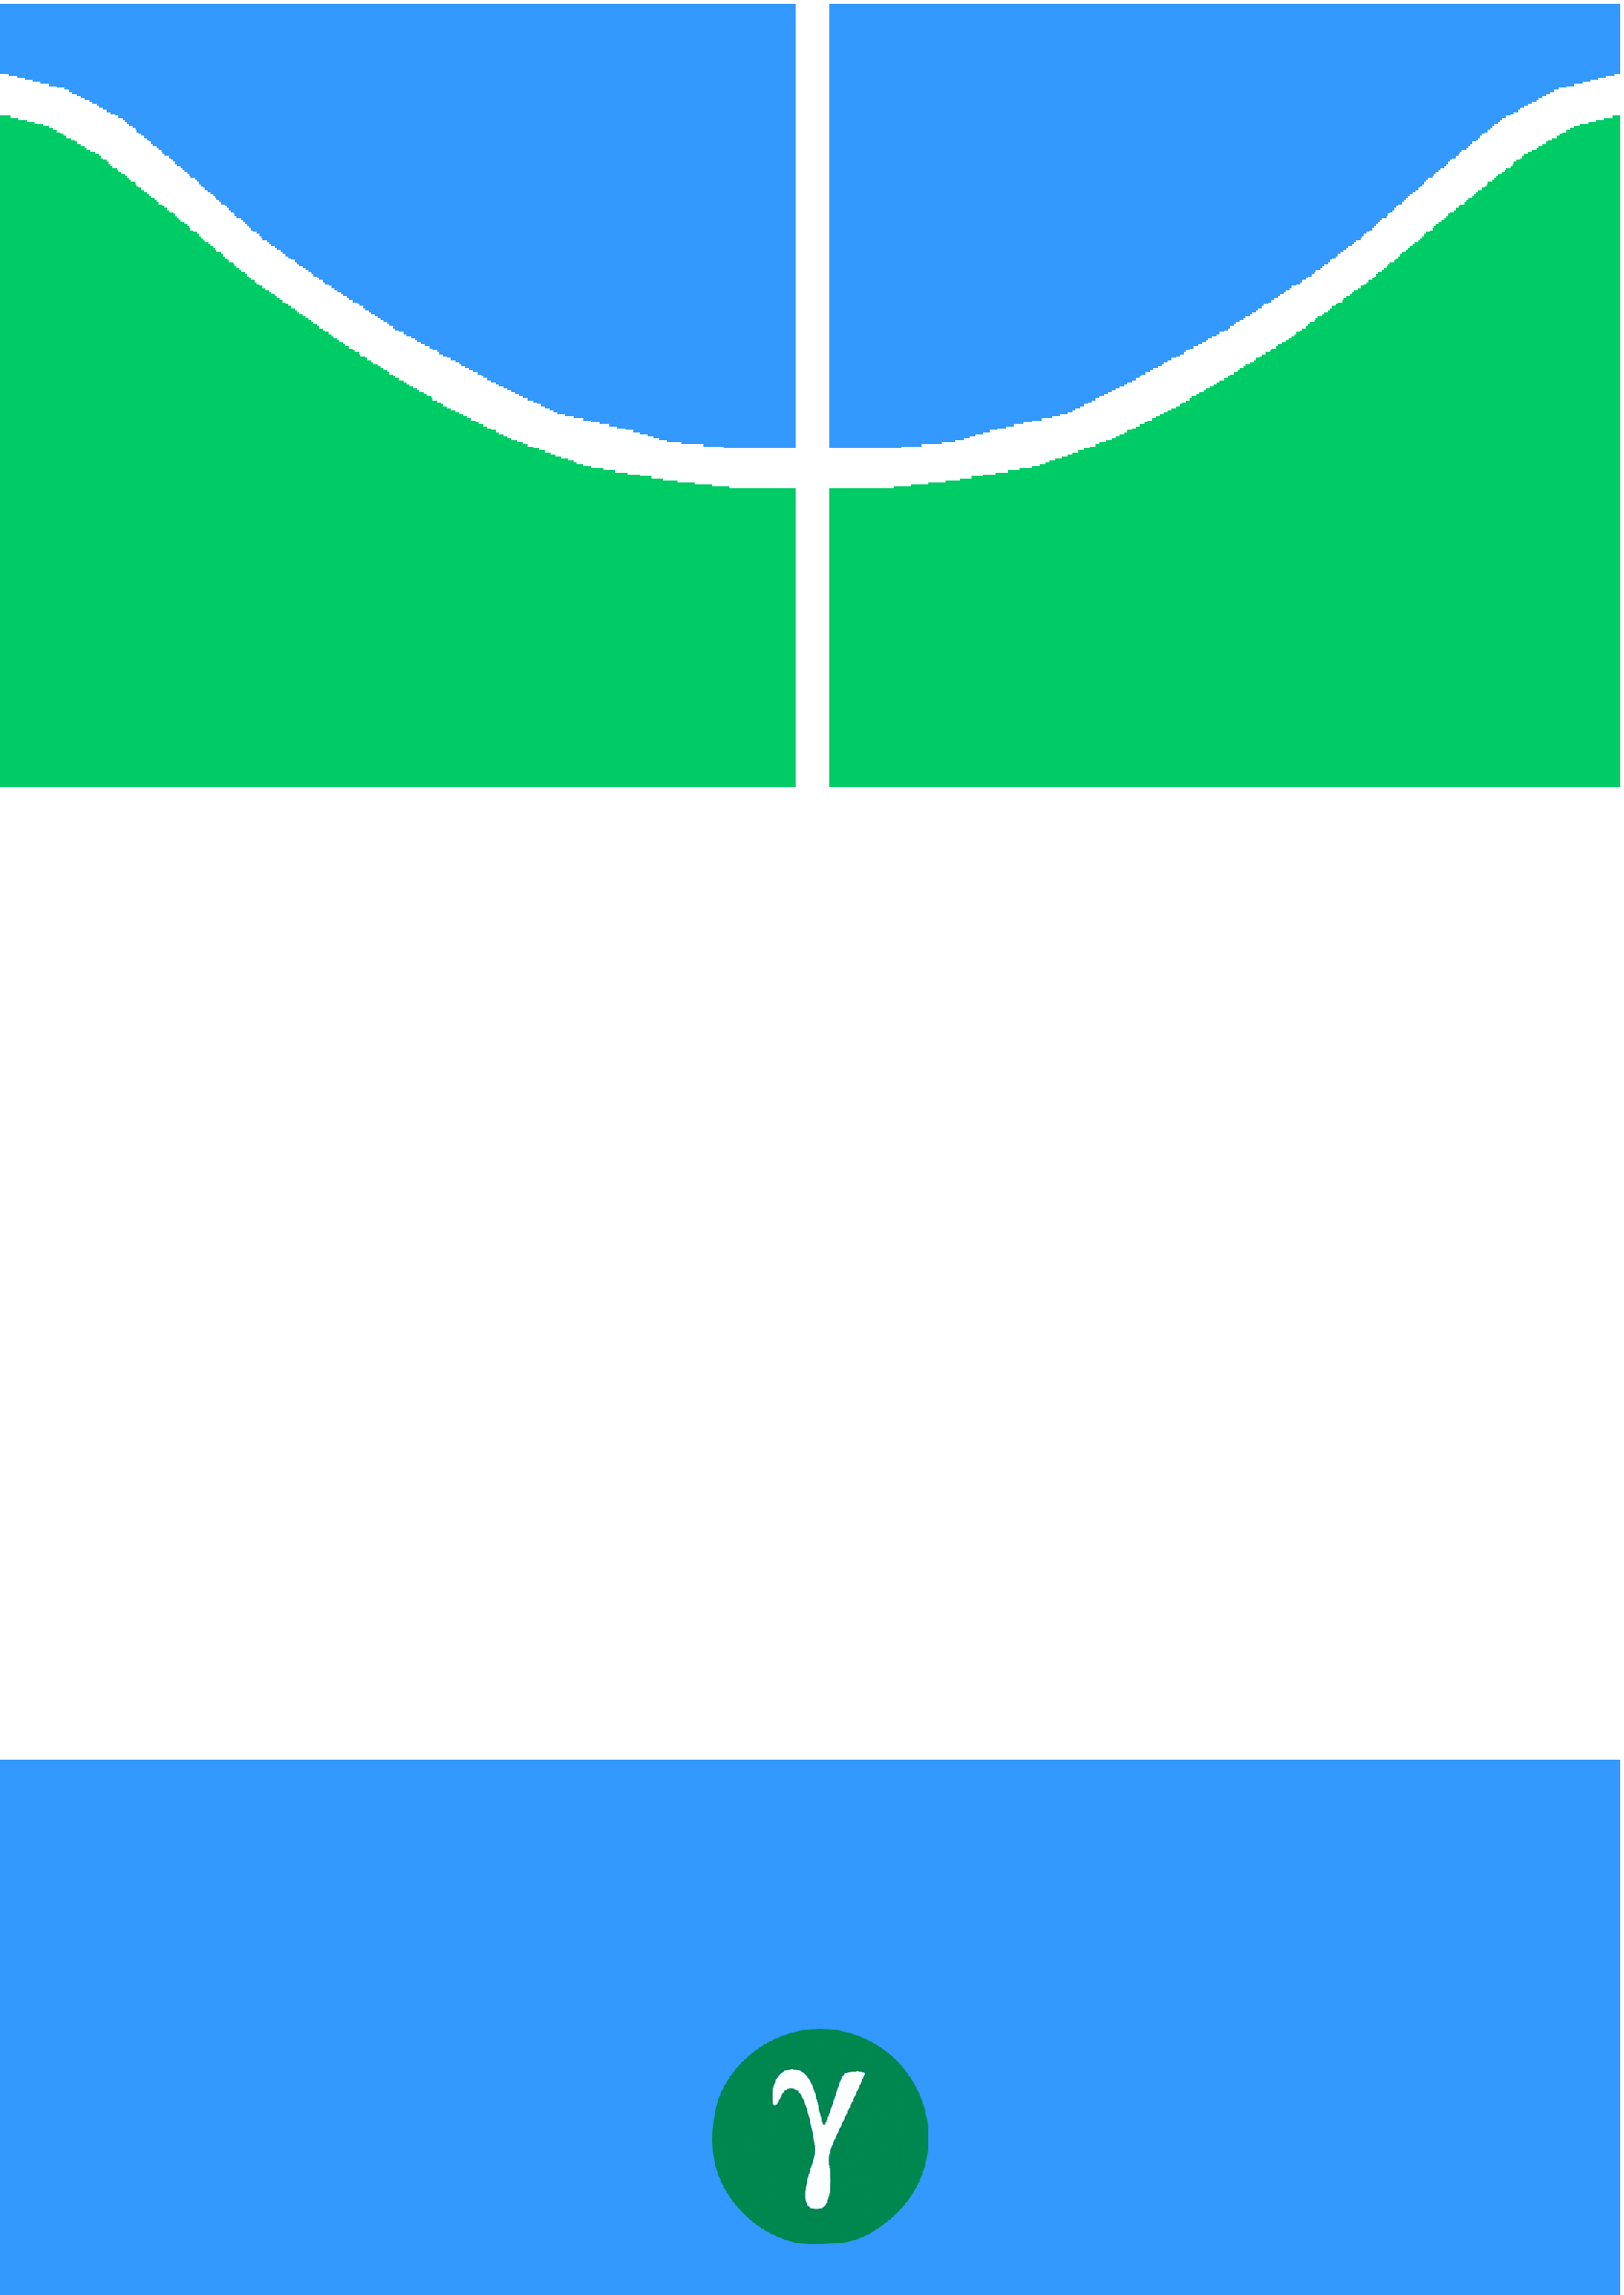
\includegraphics[width=\paperwidth,height=\paperheight,
				keepaspectratio]{capa}
			\vfill
		}
	}
}

\renewcommand{\imprimircapa}{
  \begin{capa}
    \center
	\AddToShipoutPicture*{\BackgroundPic}

    \vspace*{6.5cm}
	{\textbf{\large\imprimirinstituicao}}
	\par
	{\textbf{\large\imprimircurso}}

	\vspace*{1cm}

    {\ABNTEXchapterfont\bfseries\LARGE\imprimirtitulo}
    
	\begin{flushright}
    	\textbf{{\large{Grupo 75: \\ \imprimirautor}}}
		\par
    	\textbf{{\large{Orientador: \\ \imprimirorientador}}}
	\end{flushright}
		
    \vspace*{0.5cm}
    \textbf{{\large\imprimirlocal}}
    \par
    \textbf{{\large\imprimirdata}}
    
  \end{capa}
}

\renewcommand{\backrefpagesname}{Citado na(s) página(s):~}
\renewcommand{\backref}{}
\renewcommand*{\backrefalt}[4]{
	\ifcase #1 %
		Nenhuma citação no texto.%
	\or
		Citado na página #2.%
	\else
		Citado #1 vezes nas páginas #2.%
	\fi}%
% ---



% Dados Gerais
\autor{André Guedes, Caio Nardelli, Jonathan Moraes \\ Matheus Herlan, Matheus Oliveira e Pedro Tomioka}
\curso{Requisitos de Software - 201308 \\ Modelagem de Processos - 203921}

% Dados do trabalho
\titulo{Relatório 02 do Projeto de Melhoria CHAMEX}
\data{04 de Dezembro de 2014}

% Dados da orientacao
\orientador{George Marsicano Corrêa, MSc.}
\coorientador{}

\local{Brasília, DF}
\instituicao{
  Universidade de Brasília - UnB
  \par
  Faculdade UnB Gama - FGA
}
\tipotrabalho{Relatório de Engenharia de Software}
\preambulo{Trabalho submetido durante o curso de graduação em Engenharia de Software da Universidade de Brasília como requisito parcial para obtenção curricular da disciplina de Requisitos de \emph{Software} e Modelagem de Processos.}

\definecolor{black}{RGB}{0,0,0}
\makeatletter
\hypersetup{
		pdftitle={\@title}, 
		pdfauthor={\@author},
    	pdfsubject={\imprimirpreambulo},
		colorlinks=true,
    	linkcolor=black,
    	citecolor=black,
    	filecolor=magenta,
		urlcolor=black,
		bookmarksdepth=4
}
\makeatother
\setlength{\parindent}{1.3cm}
\setlength{\parskip}{0.2cm}  
\makeindex


\begin{document}

	\frontmatter
		\frenchspacing
		\imprimircapa
		\renewcommand{\imprimirorientadorRotulo}{ Orientador: }
		\imprimirfolhaderosto
		
		\newpage
\pdfbookmark[0]{\contentsname}{toc}
\tableofcontents*
\cleardoublepage

		\pdfbookmark[0]{\listfigurename}{lof}
\listoffigures*
\cleardoublepage
\pdfbookmark[0]{\listtablename}{lot}
\listoftables*
\cleardoublepage

		\begin{siglas}
	\item[Migue] X
\end{siglas}


	\textual

	\mainmatter

	%[RS]	Apresentar o entendimento do contexto de negócio (processo de negócio), no qual os requisitos serão identificados;
		\chapter[Contexto de Negócio]{Contexto de Negócio}
\label{chap:contexto}
	O grupo da disciplina de Requisitos de \emph{Software} (RS) ficou responsável por trabalhar, juntamente com o grupo da disciplina de Modelagem de Processos (MPR), soluções de \emph{software} para o contexto da empresa fictícia CHAMEX.
\\ \indent O objetivo da CHAMEX consiste em auxiliar pequenas e médias empresas privadas a melhorarem a qualidade de vida dos trabalhadores. Quanto mais disposição, vitalidade e alegria obtiver entre os trabalhadores, mais resultado positivo as empresas possuem.
\\ \indent Para concretização do suporte às empresas, a CHAMEX elaborou o Modelo de Avaliação (MOA). O principal objetivo desse modelo está atrelado à verificação do nível de satisfação e qualidade de vida dos funcionários de uma determinada organização. A CHAMEX apresenta um modelo de gestão por processos, tendo em vista que não há divisões de departamentos e caracterização hierárquica interna.
\\ \indent O grupo de MPR realizou um levantamento dos processos existentes dentro da CHAMEX e foram identificados:
\begin{itemize}
	\item{Inscrição no MOA;}
	\item{Seleção dos Avaliadores;}
	\item{Avaliação das Empresas;}
	\item{Validação dos Questionários;}
	\item{Compilação dos Resultados.}
\end{itemize}
\ \indent Dessa maneira, foi necessário avaliar qual dos processos descritos anteriormente seria adotado para melhoria. Assim, o grupo de MPR adotou os seguintes critérios:
\begin{itemize}
	\item{Grau de vinculação com os objetivos organizacionais ou com o direcionamento estratégico da organização;}
	\item{Impacto no cliente externo;}
	\item{Potencial para obtenção de benefícios financeiros ou redução de custos para organização;}
	\item{Impacto na imagem externa.}
\end{itemize}
\ \indent Adicionalmente, foi necessário levar em consideração a viabilidade de melhoria de cada processo. Após consideração destes fatores, o grupo de MPR chegou a conclusão de que o processo de Inscrição no MOA seria o mais apropriado para inserção de melhorias, uma vez que os outros processos apresentaram um valor de viabilidade elevado, caracterizando uma implementação complexa. O processo de Inscrição no MOA apresentou um peso significativo e um valor de viabilidade razoável.

	\section[Identificação e Descrição do Problema]{Identificação e Descrição do Problema}
	\label{sec:contexto_problema}
		Embora o processo escolhido para inserção de melhorias tenha sido a Inscrição no MOA, são apresentados, a seguir, quadros que resumem os problemas encontrados para todo o processo do MOA. É importante ressaltar que os quadros foram construídos com base nas discussões realizadas entre as equipes das disciplinas MPR e RS.

\subsection[Quadros Resumos da Descrição do Problema]{Quadros Resumos da Descrição do Problema}
\label{subsec:contexto_problema_quadros}
	\begin{table}[H]
	\centering
	\begin{tabular}{|p{6cm}|p{9cm}|}
	\hline
	O problema & Empecilhos no atendimento à demanda de solicitação de participação no MOA \\ \hline
	Afeta & Empresa CHAMEX \\ \hline
	O impacto desse problema é & As empresas que desejam participar do MOA não obtêm êxito na solicitação, inviabilizando a participação das mesmas \\ \hline
	Uma solução ideal permitiria & Informatização do processo de análise de solicitação \\ \hline
	\end{tabular}
	\label{tab:problemaUm}
	\caption[Descrição do Problema (1)]{Descrição do Problema (1).}
\end{table}
\begin{table}[H]
	\centering
	\begin{tabular}{|p{6cm}|p{9cm}|}
	\hline
	O problema & Ausência de percepção por parte da CHAMEX do processo do MOA em aplicação nas empresas \\ \hline
	Afeta & Empresa CHAMEX \\ \hline
	O impacto desse problema é & A CHAMEX não possui controle ou percepção total do que está acontecendo nas empresas durante a avaliação \\ \hline
	Uma solução ideal permitiria & Melhorias no relato do status de avaliação de cada empresa \\ \hline
	\end{tabular}
	\label{tab:problemaDois}
	\caption[Descrição do Problema (2)]{Descrição do Problema (2).}
\end{table}
\begin{table}[H]
	\centering
	\begin{tabular}{|p{6cm}|p{9cm}|}
	\hline
	O problema & Os funcionários da CHAMEX devem se locomover para as empresas participantes a fim de aplicar o MOA \\ \hline
	Afeta & Avaliadores e Empresa CHAMEX \\ \hline
	O impacto desse problema é & Os avaliadores ficam fixos em somente um contexo, não havendo flexibilidade \\ \hline
	Uma solução ideal permitiria & Interação entre avaliadores e empresas participantes pela \emph{web} \\ \hline
	\end{tabular}
	\label{tab:problemaTres}
	\caption[Descrição do Problema (3)]{Descrição do Problema (3).}
\end{table}
\begin{table}[H]
	\centering
	\begin{tabular}{|p{6cm}|p{9cm}|}
	\hline
	O problema & Os avaliadores aguardam por longos períodos de tempo o preenchimento dos questionários \\ \hline
	Afeta & Avaliadores \\ \hline
	O impacto desse problema é & Queda de produtividade para os avaliadores, visto que o tempo poderia estar sendo melhor aproveitado para realização de outras atividades \\ \hline
	Uma solução ideal permitiria & Paralelismo e sincronização de tarefas \\ \hline
	\end{tabular}
	\label{tab:problemaQuatro}
	\caption[Descrição do Problema (4)]{Descrição do Problema (4).}
\end{table}
\begin{table}[H]
	\centering
	\begin{tabular}{|p{6cm}|p{9cm}|}
	\hline
	O problema & As empresas participantes não conseguem acompanhar o status da avaliação \\ \hline
	Afeta & Empresas participantes do MOA \\ \hline
	O impacto desse problema é & Em um determinado momento, a empresa participante do MOA não consegue obter uma percepção do status de sua avaliação \\ \hline
	Uma solução ideal permitiria & Acesso imediato ao monitoramento do status da avaliação por parte da Chamex \\ \hline
	\end{tabular}
	\label{tab:problemaCinco}
	\caption[Descrição do Problema (5)]{Descrição do Problema (5).}
\end{table}

\subsection[Diagrama de \emph{Fishbone}]{Diagrama de \emph{Fishbone}}
	\label{subsec:contexto_problema_fishbone}
		Com base nos problemas identificados no processo do MOA, foi construído um Diagrama de \emph{Fishbone}, conforme descrito na Figura \ref{fig:fishbone}, de maneira a possibilitar uma boa percepção do problema principal e das causas raízes.
\begin{landscape}
	\vspace*{\fill}
	\begin{figure}[H]
		\centering
		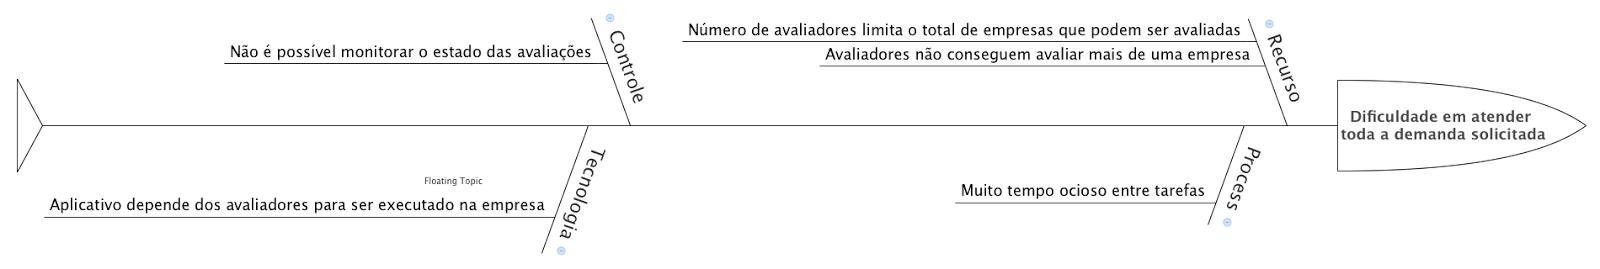
\includegraphics[scale=0.55]{fishbone}
		\caption[Diagrama de Fishbone]{Diagrama de Fishbone.}
		\label{fig:fishbone}
	\end{figure}
	\vspace*{\fill}
\end{landscape}

	\section[Processo a ser Melhorado]{Processo a ser Melhorado}
	\label{sec:contexto_problema}
		Anteriormente, no primeiro relatório do grupo de MPR, foi definido que o processo priorizado seria o processo de inscrição no MOA. A seguir será apresentada um breve resumo desse processo com o objetivo de contextualizar essa parte do projeto:

\subsection[Inscrição no MOA]{Inscrição no MOA}
\label{subsec:contexto_processoMelhorar_inscricaoMOA}
	\begin{itemize}
	\item{\textbf{Definição}: Permitir que empresas envolvidas no contexto adotado pelo MOA possam solicitar participação e consequentemente serem inscritas, caso sejam autorizadas;}
	\item{\textbf{Responsável}: CHAMEX;}
	\item{\textbf{Outros Participantes}: Empresa que deseja solicitar participação;}
	\item{\textbf{Atividades identificadas no AS-IS}:
		\begin{itemize}
			\item{\textbf{Definir Agenda do MOA}: Criar uma agenda com datas a serem cumpridas;}
			\item{\textbf{Disponibilizar Edital de Participação do MOA}: Disponibilizar edital com informações sobre o MOA;}
			\item{\textbf{Preencher Participação de Solicitação MOA}: Preencher solicitação disponibilizada pela Chamex para que seja possível participar do MOA;}
			\item{\textbf{Avaliação das Solicitações}: Identificar possíveis erros nas solicitações preenchidas pelas empresas como dados inconsistentes ou que estejam faltando;}
			\item{\textbf{Enviar Mensagem de Erro de Preenchimento}: Informar à empresa via e-mail participante quais os erros contidos no preenchimento da solicitação feita por ela;}
			\item{\textbf{Receber Mensagem de Erro de Preenchimento}: Receber via e-mail sobre os erros identificados no preenchimento da solicitação de participação no MOA;}
			\item{\textbf{Analisar Viabilidade de Participação}: Analisar se a empresa que solicitou participação no MOA está contida no contexto elaborado pela Chamex e consequentemente se ela poderá participar do MOA;}
			\item{\textbf{Enviar Resposta para a Empresa}: Informar à empresa via e-mail se ela foi autorizada a participar do MOA;}
			\item{\textbf{Receber Resposta Sobre a Viabilidade}: Receber via e-mail a resposta sobre a adesão no MOA.}
		\end{itemize}}
\end{itemize}
\begin{landscape}
	\vspace*{\fill}
	\begin{figure}[H]
		\centering
		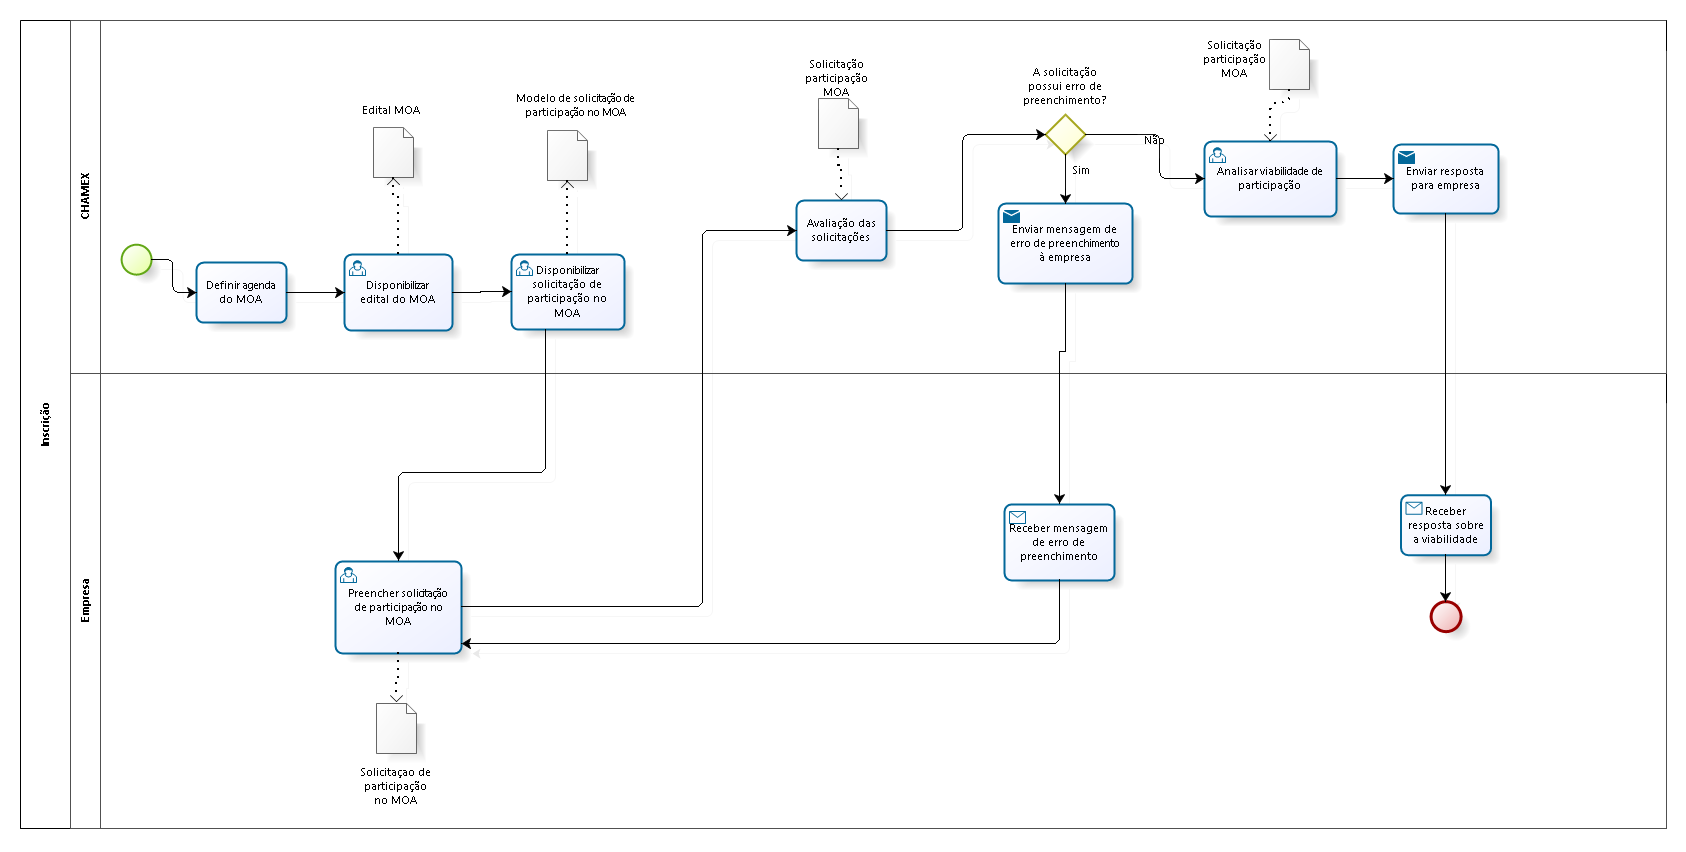
\includegraphics[scale=0.55]{inscricao_moa}
		\caption[Processo de Inscrição no MOA]{Processo de Inscrição no MOA.}
		\label{fig:processo_inscricao}
	\end{figure}
	\vspace*{\fill}
\end{landscape}

	\subsubsection[5W2H]{5W2H}
	\label{subsubsec:contexto_processoMelhorar_inscricaoMOA_5w2h}
		O 5W2H representa um conjunto de perguntas sobre um determinado processo ou atividade que procuram explicar com o máximo de clareza possível o entendimento dos colaboradores da empresa quanto ao assunto. Através das respostas extraídas nessa técnica, é possível adquirir o conhecimento necessário para criar um plano de ação que irá promover a mudança \cite{paim}.
\\ \indent O 5W representa as perguntas \emph{What?}, o que será feito; \emph{Who?}, quem irá fazer; \emph{Where?}, onde será feito; \emph{When?}, quando será feito; \emph{Why?}, porque será feito, tentando responder qual a importância daquilo para a empresa.
\\ \indent O 2H representa as perguntas \emph{How?}, como será feito; \emph{How Much?}, qual o custo relativo.

\begin{table}[H]
	\centering
	\begin{tabular}{|c|p{10cm}|}
		\hline
		\textbf{\emph{What?} O que?} & Inscrição MOA \\ \hline
		\textbf{\emph{Who?} Quem?} & CHAMEX e empresa interessada \\ \hline
		\textbf{\emph{Where?} Onde?} & Empresa CHAMEX e site CHAMEX \\ \hline
		\textbf{\emph{When?} Quando?} & Inicio do período de inscrição \\ \hline
		\textbf{\emph{Why?} Por quê?} & Passo inicial necessário para saber quais empresas vão participar do MOA \\ \hline
		\textbf{\emph{How?} Como?} & Empresas se inscrevem no MOA a partir de uma planilha disponibilizada no site da CHAMEX \\ \hline
		\textbf{\emph{How Much?} Quanto?} & - \\ \hline
	\end{tabular}
	\label{tab:5w2h}
	\caption[5W2H no Contexto de Inscrição no MOA]{5W2H no Contexto de Inscrição no MOA.}
\end{table}

	\section[Simulação AS-IS]{Simulação AS-IS}
	\label{sec:contexto_asis}
		Para a simulação dos processos foi escolhido o processo mais viável a ser tratado da lista de processos da CHAMEX, e também os dois processos de maior valor numérico de prioridade da mesma. Assim será simulado os processos de Inscrição no MOA (mais viável). O tempo de execução e o número de cada tarefa foi baseado no \emph{feedback} do cliente e em casos onde não foi possível haver o conhecimento de tal, foram estimados os dados de acordo com o consenso da equipe de modelagem do processo.
\\ A seguir serão listadas as configurações e resultados para os cenários de simulação.

\subsection[Propriedades dos Cenários de Simulação]{Propriedades dos Cenários de Simulação}
\label{subsec:contexto_asis_cenarios}
	\begin{itemize}
	\item{\textbf{Cenário 1}:
		\begin{itemize}
			\item{\textbf{Duração}: 30 Dias;}
			\item{\textbf{Unidade Básica de Medida}: Horas;}
			\item{\textbf{Instâncias Iniciadas}: 10.}
		\end{itemize}}
	\item{\textbf{Cenário 2}:
		\begin{itemize}
			\item{\textbf{Duração}: 30 Dias;}
			\item{\textbf{Unidade Básica de Medida}: Horas;}
			\item{\textbf{Instâncias Iniciadas}: 30.}
		\end{itemize}}
	\item{\textbf{Recursos Disponíveis}:
		\begin{itemize}
			\item{\textbf{Gerente}: 1;}
			\item{\textbf{Avaliador}: 5;}
			\item{\textbf{Empresa}: 10;}
		\end{itemize}}
\end{itemize}

\subsection[Recursos e Tempo de Processamento do Cenário de Simulação]{Recursos e Tempo de Processamento do Cenário de Simulação}
\label{subsec:contexto_asis_tempo}
	\begin{table}[H]
	\centering
	\begin{tabular}{|p{5cm}|c|c|c|}
		\hline
		\textbf{Atividade} & \textbf{Recurso} & \textbf{Quantidade} & \textbf{Horas} \\ \hline
		Analisar viabilidade de participação & Analista & 1 & 4 \\ \hline
		Avaliação das solicitações & Analista & 1 & 4 \\ \hline
		Definir agenda do MOA & Gerente & 1 & 24 \\ \hline
		Disponibilizar solicitação de participação no MOA & Gerente & 1 & 1.16 \\ \hline
		Disponibilizar edital do MOA & Gerente & 1 & 8 \\ \hline
		Enviar mensagem de erro de preenchimento à empresa & Analista & 1 & 0.5 \\ \hline
		Enviar resposta para empresa & Analista & 1 & 0.5 \\ \hline
		Preencher solicitação de participação no MOA & Empresa & 1 & 48 \\ \hline
		Receber mensagem de erro de preenchimento & Empresa & 1 & 0.16 \\ \hline
		Receber resposta sobre a viabilidade & Empresa & 1 & 0.16 \\ \hline
	\end{tabular}
	\caption[Recursos e Tempo de Processamento do Cenário de Simulação]{Recursos e Tempo de Processamento do Cenário de Simulação}
\end{table}

\subsection[Resultado da Simulação]{Resultado da Simulação}
\label{subsec:contexto_asis_resultado}
	O tempo total médio do processo foi de 231.17 horas para o cenário 1 e 627.83 horas para o 2. A Figura \ref{fig:resultadosasis} apresenta os resultados da simulação.
\begin{figure}[H]
	\centering
	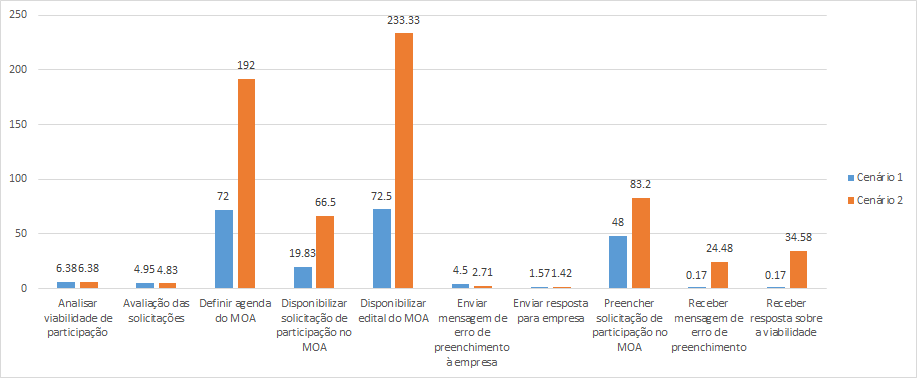
\includegraphics[scale=0.66]{resultado_asis_simulacao}
	\caption[Gráfico de Resultados da Simulação AS-IS]{Gráfico de Resultados da Simulação AS-IS.}
	\label{fig:resultadosasis}
\end{figure}

\subsection[Recursos]{Recursos}
\label{subsec:contexto_asis_recursos}
	\begin{figure}[H]
	\centering
	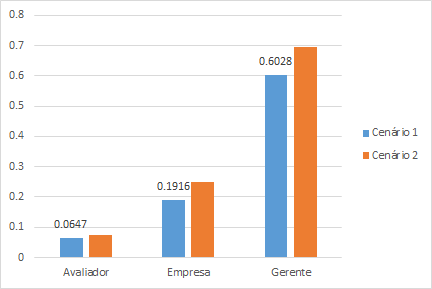
\includegraphics[scale=1]{recursos_asis_simulacao}
	\caption[Gráfico de Recursos da Simulação AS-IS]{Gráfico de Recursos da Simulação AS-IS.}
	\label{fig:recursosasis}
\end{figure}

\subsection[Análise do Resultado]{Análise do Resultado}
\label{subsec:contexto_asis_analise}
	Para ambos os cenários as atividade Definir Agenda do MOA, Disponibilizar Solicitação de Participação no MOA e Disponibilizar Edital do MOA apresentaram um valor mais elevado quanto a média de horas das demais atividades, isso resultou no alto valor para utilização do Gerente no processo.
\\ \indent As demais atividades apresentaram valores próximos do esperado no Cenário 1. No Cenário 2 o tempo foi discrepante devido ao gargalo gerado pelas atividades iniciais do gerente, que acabam influenciando todas as demais. A baixa utilização do analista se mostra preocupante, pois se espera que ele utilize mais o tempo do processo avaliando as solicitações.
	%[RS]	Aplicar ao menos duas técnicas de elicitação de requisitos;
		\chapter[Resultados Obtidos: Técnicas de Elicitação]{Resultados Obtidos: Técnicas de Elicitação}
\label{chap:elicitacao}
	Primeiramente, é importante ressaltar que a elicitação remete ao significado de descobrimento. De maneira geral, cabe à elicitação a tarefa de identificar os fatos relacionados aos requisitos do sistema, de maneira a prover o mais correto e completo entendimento acerca do que é demandado pelo \emph{software} que está sendo concebido.
\\ \indent Mediante às informações apresentadas anteriormente, é necessário afirmar que a fase de levantamento de requisitos necessita de suporte para que possa ser executada com êxito.
\\ \indent Assim sendo, a partir da abordagem adotada pelo time, de natureza adaptativa, as seguintes técnicas de elicitação foram escolhidas:
\begin{itemize}
	\item{\textbf{\emph{Brainstorming}}: Técnica que consiste em reuniões para a geração de ideias, onde até as ideias não convencionais são encorajadas para a agregação do maior número de ideias possíveis para serem revisadas e escolhidas, favorecendo o surgimento de soluções criativas para o problema. No âmbito do projeto, todas as reuniões realizadas várias ideias para resolução da problemática eram apresentadas. Ao final da apresentação das sugestões, todas as propostas eram discutidas. Um momento decisivo para utilização do \emph{brainstorming} no contexto do projeto esteve atrelado à formalização dos campos que seriam solicitados no formulário de solicitação de participação do MOA e também, nas perguntas constituintes do \emph{check-list} da solicitação do MOA.}
	\item{\textbf{Prototipagem}: Técnica muito utilizada na elicitação de requisitos, pois possibilita uma visão prática, condizente ou não com o produto final baseado no seu nível de fidelidade, que facilita a interpretação concreta dos critérios a serem atingidos para a aceitação da porção da solução na qual a técnica foi utilizada. No âmbito do projeto, facilitou a interpretação concreta dos critérios a serem atingidos para a aceitação da porção da solução onde foi utilizada.
	\\ \indent Por meio das reuniões que foram realizadas, muitos aspectos eram apresentados para discussão. No momento anterior à criação da solução de BPMS, foram discutidas características da solução. Dessa maneira, foi construído um protótipo de baixa fidelidade para favorecer o entendimento.
	\begin{figure}[H]
		\centering
		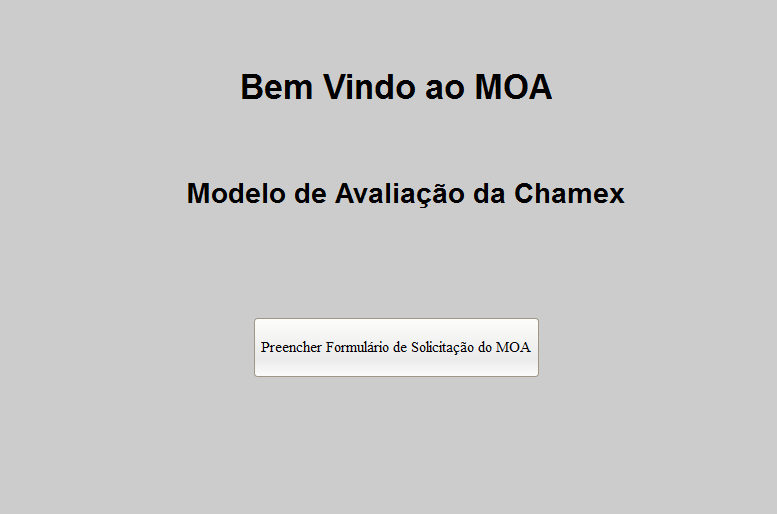
\includegraphics[scale=0.55]{prototipo_1}
		\caption[Protótipo da Página Inicial da Solução]{Protótipo da Página Inicial da Solução.}
		\label{fig:protipoum}
	\end{figure}
	\begin{figure}[H]
		\centering
		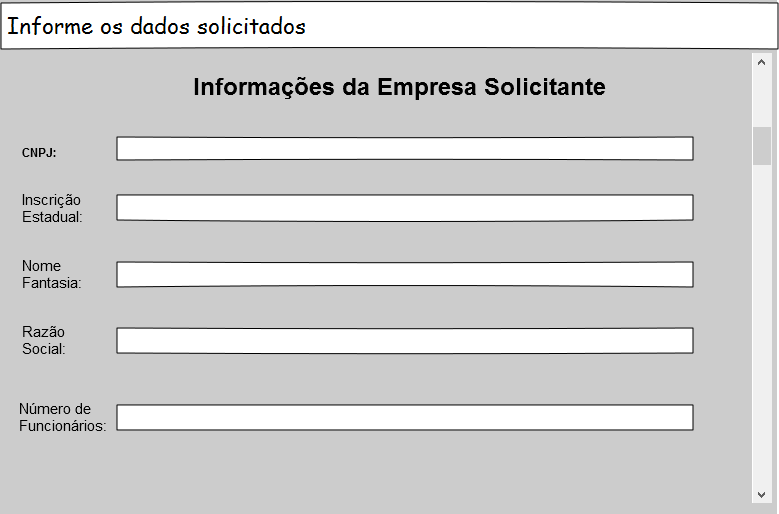
\includegraphics[scale=0.55]{prototipo_2}
		\caption[Protótipo da Primeira Página do Formulário de Inscrição]{Protótipo da Primeira Página do Formulário de Inscrição.}
		\label{fig:protipodois}
	\end{figure}
	\begin{figure}[H]
		\centering
		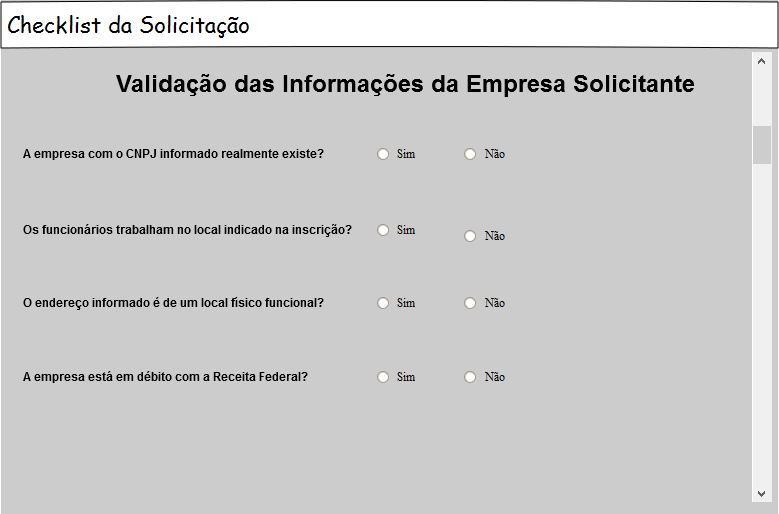
\includegraphics[scale=0.55]{prototipo_3}
		\caption[Protótipo da Página do \emph{Check-list}]{Protótipo da Página do \emph{Check-list}.}
		\label{fig:protipotres}
	\end{figure}}
\end{itemize}

	%[RS]	De acordo com a estratégia a ser utilizada pelo grupo: identificar e descrever o problema, as necessidades, as características, casos de uso, users stories, temas de investimento, épicos, requisitos funcionais e requisitos não funcionais;
	%[RS]	Detalhar user stories / casos de uso (referentes à primeira iteração do projeto);
		\chapter[Definições de Requisitos Ágeis]{Definições de Requisitos Ágeis}
\label{chap:requisitos}
	\section[Levantamento de Requisitos]{Levantamento de Requisitos}
	\label{sec:requisitos_levantamento}
		\subsection[Nível de Portfólio]{Nível de Portfólio}
\label{subsec:requisitos_levantamento_portfolio}
	\begin{itemize}
		\item{\textbf{Tema de Investimento}: Modelo de Avaliação (MOA)
			\\ Referência: Macro-Processo \cite{moa}}
		\item{\textbf{Épicos}:
			\begin{itemize}
				\item{\textbf{PT01}: Administração do MOA
				\\ Referência: Processo de Inscrição do MOA \& Seleção dos Avaliadores}
				\item{\textbf{PT02}: Solicitação do MOA
				\\ Referência: Processo de Inscrição do MOA}
				\item{\textbf{PT03}: Questionários do MOA
				\\ Referência: Avaliação das Empresas \& Validação dos Questionários \& Compilação dos Resultados}
				\item{\textbf{PT04}: Rede de Interação do MOA
				\\ Referência: Macro-Processo}
			\end{itemize}}
	\end{itemize}

\subsection[Nível de Programa]{Nível de Programa}
\label{subsec:requisitos_levantamento_programa}
	\begin{itemize}
		\item{\textbf{\emph{Features}}:
			\begin{itemize}
				\item{\textbf{PR0101}: Geração de Agenda do MOA
				\\ Referência: PT01, Processo de Inscrição do MOA}
				\item{\textbf{PR0102}: Geração de Edital do MOA
				\\ Referência: PT01, Processo de Inscrição do MOA}
				\item{\textbf{PR0103}: Gestão de Avaliadores do MOA
				\\ Referência: PT01, Processo de Inscrição do MOA \& Seleção dos Avaliadores}
				\item{\textbf{PR0201}: Solicitação de Participação no MOA
				\\ Referência: PT02, Processo de Inscrição do MOA}
				\item{\textbf{PR0202}: Validação de Solicitação de Participação no MOA
				\\ Referência: PT02, Processo de Inscrição do MOA}
				\item{\textbf{PR0301}: Aplicação de Questionários do MOA
				\\ Referência: PT03, Avaliação das Empresas \& Validação dos Questionários}
				\item{\textbf{PR0302}: Análise de Questionários do MOA
				\\ Referência: PT03, Validação dos Questionários}
				\item{\textbf{PR0303}: Disponibilização de Resultados do MOA
				\\ Referência: PT03, Compilação dos Resultados}
				\item{\textbf{PR0401}: Perfis de Interação do MOA
				\\ Referência: PT04, Macro-Processo}
				\item{\textbf{PR0402}: Grupos de Interação do MOA
				\\ Referência: PT04, Macro-Processo}
			\end{itemize}}
	\end{itemize}

\subsection[Nível de Time do Épico PT02]{Nível de Time do Épico PT02}
\label{subsec:requisitos_levantamento_programa}
	\begin{itemize}
		\item{\textbf{Histórias de Usuário}:
			\begin{itemize}
				\item{\textbf{T020101}: Eu como representante da empresa solicitante desejo preencher  o formulário de solicitação do MOA para registrar a intenção de participação da empresa que represento.
				\\ \textbf{Critérios de Aceitação}
				\begin{enumerate}
					\item{O formulário deverá solicitar os seguintes itens da Empresa Solicitante:
					\begin{itemize}
						\item{CNPJ}
						\item{Data de Deferimento}
						\item{Inscrição Estadual}
						\item{Nome Fantasia}
						\item{Razão Social}
						\item{Número de Funcionários}
						\item{Área de Atuação}
						\item{Renda Média Anual}
						\item{Endereço com os seguintes campos: Bairro, Cidade, UF, Número, Complemento, CEP}
						\item{Telefone para contato}
						\item{E-mail}
						\item{Número de Estabelecimentos}
						\item{Participação em Processos de Avaliação com os seguintes campos: Informações sobre o Processo de Avaliação que já participou e quais foram as Instituições Avaliadoras; Em caso de não participação, informar se já se inscreveu e nunca foi contemplado}
					\end{itemize}}
					\item{Quanto ao preenchimento do formulário, os seguintes dados serão obrigatórios:
					\begin{itemize}
						\item{CNPJ}
						\item{Data de Deferimento}
						\item{Inscrição Estadual}
						\item{Razão Social}
						\item{Número de Funcionários}
						\item{Área de Atuação}
						\item{Os seguintes campos de Endereço: Bairro, Cidade, UF, Número, CEP}
						\item{Telefone para contato}
						\item{E-mail}
					\end{itemize}}
					\item{Para participar, a Empresa Solicitante deverá conter, no mínimo, 10 funcionários.}
				\end{enumerate}
				Referência: PR0201, Processo de Inscrição do MOA}
				\item{\textbf{T020102}: Eu como gerente de solicitação do MOA desejo atribuir solicitações à um determinado analista de solicitação para responsabilizar o analista pela validação da solicitação.
				\\ \textbf{Critérios de Aceitação}
				\begin{enumerate}
					\item{Deverá estar disponível uma lista de solicitações enviadas pelas empresas solicitantes.}
					\item{Deverá estar disponível uma lista de analistas de solicitações.}
					\item{Deverá ser possível atribuir uma solicitação a um analista de solicitações.}
					\item{Apenas um analista de solicitações deverá estar vinculado a uma solicitação.}
					\item{O gerente de solicitações poderá atribuir até 50 solicitações simultâneas à um determinado analista de solicitações.}
				\end{enumerate}
				Referência: PR0201, Processo de Inscrição do MOA}
				\item{\textbf{T020103}: Eu como representante da empresa solicitante desejo cancelar a solicitação de participação para informar a intenção de desistência.
				\\ \textbf{Critérios de Aceitação}
				\begin{enumerate}
					\item{Deverá ser possível cancelar a solicitação de participação até 48 horas antes do término das inscrições.}
					\item{Uma vez cancelada a solicitação de participação, não deverá ser possível reatar a intenção de participação para o edital corrente.}
				\end{enumerate}
				Referência: PR0201, Processo de Inscrição do MOA}
				\item{\textbf{T020201}: Eu como analista de solicitação do MOA desejo selecionar uma solicitação de participação do MOA para definir qual solicitação será validada.
				\\ \textbf{Critérios de Aceitação}
				\begin{enumerate}
					\item{O analista de solicitações poderá escolher uma e somente uma solicitação para validação por vez.}
					\item{O analista de solicitações não poderá escolher uma nova solicitação para validação enquanto estiver com uma solicitação escolhida pendente.}
				\end{enumerate}
				Referência: PR0202, Processo de Inscrição do MOA}
				\item{\textbf{T020202}: Eu como analista de solicitação do MOA desejo validar os dados fornecidos pela empresa solicitante para determinar a viabilidade de participação.
				\\ \textbf{Critérios de Aceitação}
				\begin{enumerate}
					\item{Deverá haver um Checklist para controle da avaliação da solicitação por parte do analista de solicitações e um campo para envio de considerações quanto à solicitação.}
					\item{O Checklist deverá incluir os seguintes questionamentos:
					\begin{itemize}
						\item{A Empresa com o CNPJ informado realmente existe?}
						\item{Os funcionários trabalham no local indicado na solicitação?}
						\item{O número de funcionários que trabalham na empresa está dentro do valor estipulado?}
						\item{O endereço informado é de um local físico funcional?}
						\item{O telefone informado pertence à Empresa solicitante?}
						\item{A área de atuação corresponde à mesma do período corrente do MOA?}
						\item{A Empresa solicitante está em débito com a Receita Federal?}
						\item{O e-mail informado realmente pertence à Empresa solicitante?}
 					\end{itemize}}
					\item{Deverá ser disponibilizada a opção de reprovar uma solicitação.}
					\item{Deverá ser disponibilizada a opção de aprovar uma solicitação.}
					\item{Deverá ser disponibilizada a opção para enviar a solicitação para correção.}
				\end{enumerate}
				Referência: PR0202, Processo de Inscrição do MOA}
				\item{\textbf{T020203}: Eu como representante da empresa solicitante desejo alterar as informações do formulário de solicitação de participação do MOA para corrigir inconsistências encontradas pelo analista de solicitação.
				\\ \textbf{Critérios de Aceitação}
				\begin{enumerate}
					\item{O representante da empresa solicitante só poderá efetuar correções no formulário de solicitação caso a mesma seja passível de correções.}
					\item{Os itens só poderão ser modificados se exigida a devida correção.}
				\end{enumerate}
				Referência: PR0202, Processo de Inscrição do MOA}
			\end{itemize}}
	\end{itemize}

	\section[Priorização de Requisitos]{Priorização de Requisitos}
	\label{sec:requisitos_priorizacao}
		\subsection[Visão Geral]{Visão Geral}
\label{subsec:requisitos_priorizacao_geral}
	\begin{figure}[H]
		\centering
		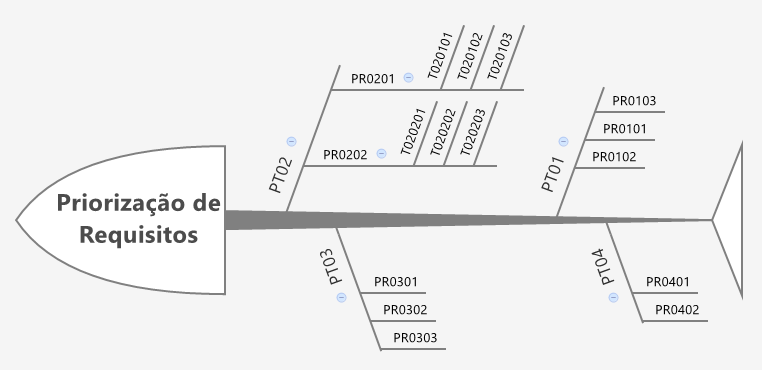
\includegraphics[scale=0.5]{priorizacao_requisitos}
		\caption[Visão Geral de Requisitos Priorizados do MOA]{Visão Geral de Requisitos Priorizados do MOA.}
		\label{fig:visaogeralpriorizado}
	\end{figure}

\subsection[Épicos no Nível de Portfólio]{Épicos no Nível de Portfólio}
\label{subsec:requisitos_priorizacao_portfolio}
	\subsubsection[Atributos]{Atributos}
	\label{subsubsec:requisitos_priorizacao_portfolio_atributos}
		\begin{itemize}
			\item{\textbf{PT01}: Administração do MOA
			\\ Prioridade: Importante
			\\ Estabilidade: Média
			\\ Risco: Baixo}
			\item{\textbf{PT02}: Solicitação do MOA
			\\ Prioridade: Essencial
			\\ Estabilidade: Alta
			\\ Risco: Baixo}
			\item{\textbf{PT03}: Questionários do MOA
			\\ Prioridade: Essencial
			\\ Estabilidade: Alta
			\\ Risco: Baixo}
			\item{\textbf{PT04}: Rede de Interação do MOA
			\\ Prioridade: Desejável
			\\ Estabilidade: Média
			\\ Risco: Baixo}
		\end{itemize}

	\subsubsection[Sequência Linear]{Sequência Linear}
	\label{subsubsec:requisitos_priorizacao_portfolio_sequencia}
		\begin{center}
		$PT02 \rightarrow PT03 \rightarrow PT01 \rightarrow PT04$
		\end{center}

\subsection[\emph{Features} no Nível de Programa]{\emph{Features} no Nível de Programa}
\label{subsec:requisitos_priorizacao_programa}
	\subsubsection[Atributos]{Atributos}
	\label{subsubsec:requisitos_priorizacao_programa_atributos}
		\begin{itemize}
			\item{\textbf{PR0101}: Geração de Agenda do MOA
			\\ Prioridade: Desejável
			\\ Estabilidade: Média
			\\ Risco: Baixo}
			\item{\textbf{PR0102}: Geração de Edital do MOA
			\\ Prioridade: Desejável
			\\ Estabilidade: Média
			\\ Risco: Baixo}
			\item{\textbf{PR0103}: Gestão de Avaliadores do MOA
			\\ Prioridade: Importante
			\\ Estabilidade: Alta
			\\ Risco: Médio}
			\item{\textbf{PR0201}: Solicitação de Participação no MOA
			\\ Prioridade: Essencial
			\\ Estabilidade: Alta
			\\ Risco: Baixo}
			\item{\textbf{PR0202}: Validação de Solicitação de Participação no MOA
			\\ Prioridade: Essencial
			\\ Estabilidade: Alta
			\\ Risco: Baixo}
			\item{\textbf{PR0301}: Aplicação de Questionários do MOA
			\\ Prioridade: Essencial
			\\ Estabilidade: Alta
			\\ Risco: Baixo}
			\item{\textbf{PR0302}: Análise de Questionários do MOA
			\\ Prioridade: Essencial
			\\ Estabilidade: Média
			\\ Risco: Médio}
			\item{\textbf{PR0303}: Disponibilização de Resultados do MOA
			\\ Prioridade: Desejável
			\\ Estabilidade: Baixa
			\\ Risco: Baixo}
			\item{\textbf{PR0401}: Perfis de Interação do MOA
			\\ Prioridade: Desejável
			\\ Estabilidade: Baixa
			\\ Risco: Alto}
			\item{\textbf{PR0402}: Grupos de Interação do MOA
			\\ Prioridade: Desejável
			\\ Estabilidade: Baixa
			\\ Risco: Alto}
		\end{itemize}

	\subsubsection[Sequência Linear]{Sequência Linear}
	\label{subsubsec:requisitos_priorizacao_programa_sequencia}
		\begin{center}
		$PR0201 \rightarrow PR0202 \rightarrow PR0301 \rightarrow PR0302 \rightarrow PR0303 \rightarrow$
		\\
		$PR0103 \rightarrow PR0101 \rightarrow PR0102 \rightarrow PR0401 \rightarrow PR0402$
		\end{center}

\subsection[Histórias de Usuário no Nível de Time do Épico PT02]{Histórias de Usuário no Nível de Time do Épico PT02}
\label{subsec:requisitos_priorizacao_programa}
	\subsubsection[Atributos]{Atributos}
	\label{subsubsec:requisitos_priorizacao_time_atributos}
		\begin{itemize}
			\item{\textbf{T020101}
			\\ Prioridade: Essencial
			\\ Estabilidade: Alta
			\\ Risco: Médio
			\\ Responsável: Matheus Herlan}
			\item{\textbf{T020102}
			\\ Prioridade: Essencial
			\\ Estabilidade: Média
			\\ Risco: Baixo
			\\ Responsável: André Guedes}
			\item{\textbf{T020103}
			\\ Prioridade: Importante
			\\ Estabilidade: Alta
			\\ Risco: Baixo
			\\ Responsável: Caio Nardelli}
			\item{\textbf{T020201}
			\\ Prioridade: Importante
			\\ Estabilidade: Média
			\\ Risco: Baixo
			\\ Responsável: Caio Nardelli}
			\item{\textbf{T020202}
			\\ Prioridade: Essencial
			\\ Estabilidade: Alta
			\\ Risco: Médio
			\\ Responsável: Jonathan Moraes}
			\item{\textbf{T020203}
			\\ Prioridade: Importante
			\\ Estabilidade: Alta
			\\ Risco: Médio
			\\ Responsável: Matheus Herlan}
		\end{itemize}

	\subsubsection[Sequência Linear]{Sequência Linear}
	\label{subsubsec:requisitos_priorizacao_time_sequencia}
		\begin{center}
		$T020101 \rightarrow T020102 \rightarrow T020103 \rightarrow T020202 \rightarrow T020203 \rightarrow T020201$
		\end{center}

	\section[\emph{Roadmap}]{\emph{Roadmap}}
	\label{sec:requisitos_roadmap}
		\begin{figure}[H]
	\centering
	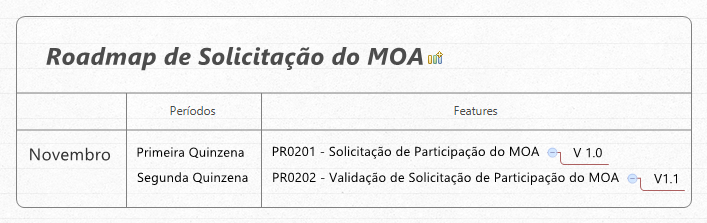
\includegraphics[scale=0.65]{roadmap_requisitos}
	\caption[Roadmap do Épico Solicitação do MOA]{Roadmap do Épico Solicitação do MOA.}
	\label{fig:roadmap}
\end{figure}
	%[MPR]	Identificar pontos de automatização e melhoria do processo;
		\chapter[Modelagem TO-BE do Processo de Inscrição no MOA]{Modelagem TO-BE do Processo de Inscrição no MOA}
\label{chap:processotobe}
	Esse capítulo tem como objetivo apresentar a modelagem do modelo TO-BE para o processo de inscrição, apresentando quais os passos que foram seguidos para elaborar essa nova modelagem.

	\section[Suprimir Atividades Redundantes e Sem Propósito Claro]{Suprimir Atividades Redundantes e Sem Propósito Claro}
	\label{sec:processotobe_suprimir}
		Analisando o processo AS-IS, as seguintes atividades foram julgadas como redundantes ou sem propósito claro e foram removidas:
\begin{itemize}
	\item{\textbf{Definir Agenda MOA}: Não possui propósito claro dentro do contexto de inscrição;}
	\item{\textbf{Disponibilizar Edital do MOA}: Não possui valor real para o processo de inscrição, visto que pode ter sido realizada anteriormente.}
\end{itemize}
\begin{figure}[H]
	\centering
	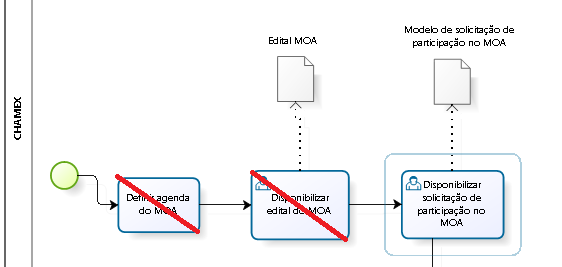
\includegraphics[scale=1]{remover_atividades_1}
	\label{fig:atividaderemovidaum}
	\caption[Atividades Removidas pelo Critério de Redundância]{Atividades Removidas pelo Critério de Redundância.}
\end{figure}

	\section[Melhora do Sequenciamento dos Passos e Simplificação de Atividades Complexas]{Melhora do Sequenciamento dos Passos e Simplificação de Atividades Complexas}
	\label{sec:processotobe_simplificar}
		Em uma análise de como os passos seriam sequenciados de uma maneira mais clara e simplificada, as atividades de envio e recebimento de mensagens acerca do status da solicitação foram substituídas por uma atividade de consulta de dados realizada pela própria empresa. 
\\ \indent Imaginando que cabe à empresa a decisão sobre corrigir os erros ou desistir da participação, foi criada uma atividade onde a viabilidade da correção dos erros é colocada em pauta, com um gateway que indica qual a decisão tomada.
\\ \indent A Figura \ref{fig:atividaderemovidadois} apresenta a remoção das atividades relacionadas a envio e recebimento de mensagem sobre o status do AS-IS para criação do TO-BE.
\begin{figure}[H]
	\centering
	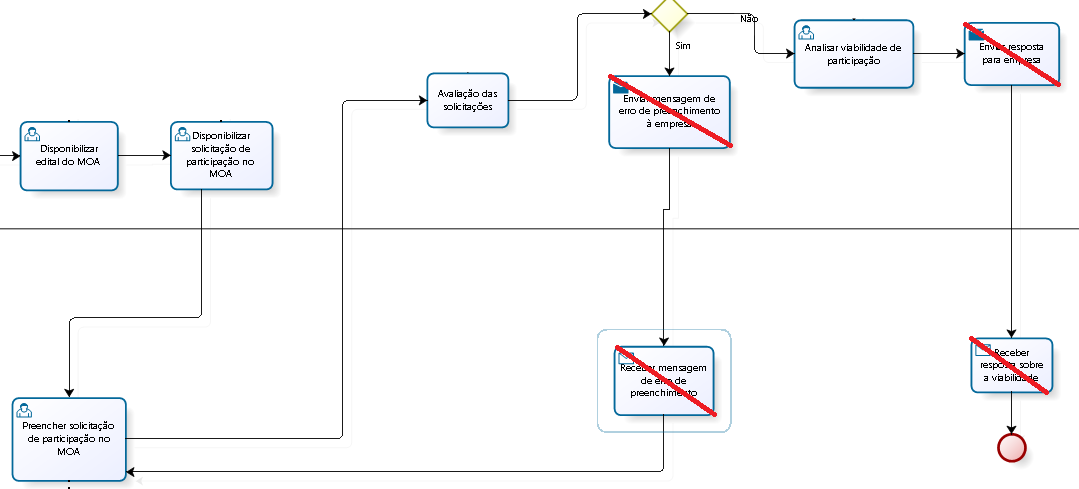
\includegraphics[scale=0.5]{remover_atividades_2}
	\caption[Atividades Removidas pelo Critério de Simplificação]{Atividades Removidas pelo Critério de Simplificação.}
	\label{fig:atividaderemovidadois}
\end{figure}
A Figura \ref{fig:atividaderemovidatres} apresenta a inclusão de atividades desenvolvidas pelas empresas solicitantes que melhoram e simplificam o sequenciamento das atividades logo após análise da viabilidade da participação da empresa pela CHAMEX:
\begin{figure}[H]
	\centering
	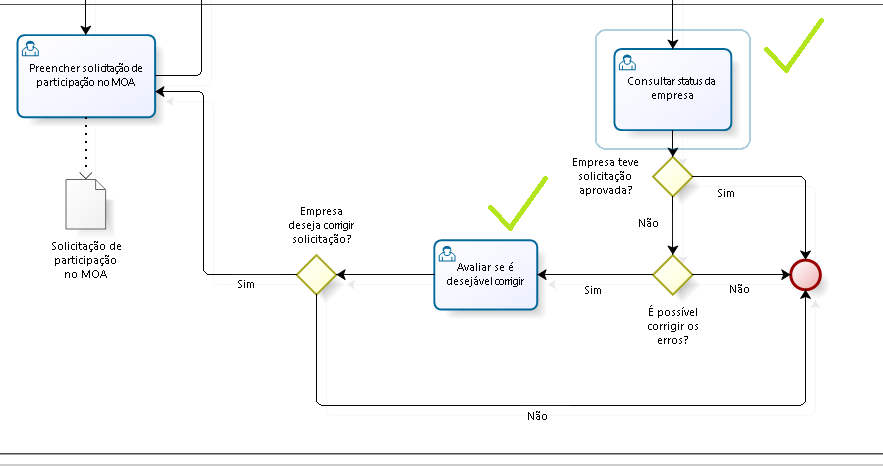
\includegraphics[scale=0.6]{remover_atividades_3}
	\caption[Inclusão de Atividades pelo Critério de Melhoria de Sequenciamento]{Inclusão de Atividades pelo Critério de Melhoria de Sequenciamento.}
	\label{fig:atividaderemovidatres}
\end{figure}

	\section[Modelagem Final do TO-BE]{Modelagem Final do TO-BE}
	\label{sec:processotobe_final}
		Baseando-se nos passos anteriores, onde atividades foram excluídas e incluídas, simplificando o sequenciamento do processo bem como facilitando seu entendimento, o seguinte modelo TO-BE foi desenvolvido por completo na sua primeira versão:
\begin{figure}[H]
	\centering
	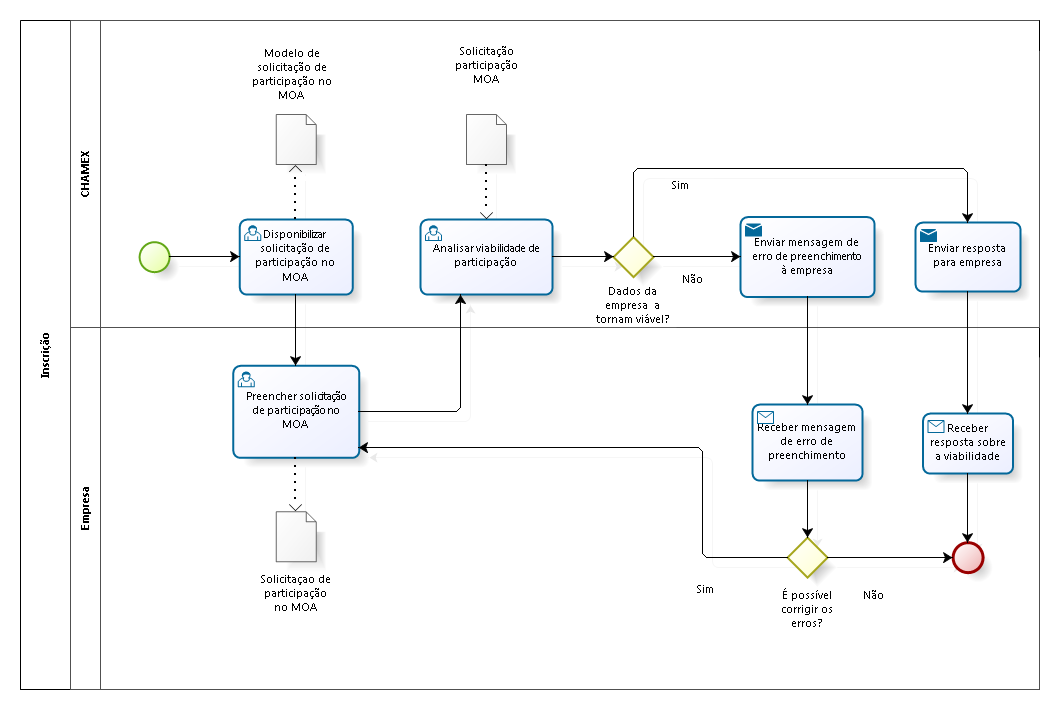
\includegraphics[scale=0.55]{to-be_1}
	\label{fig:tobeversaoum}
	\caption[Primeira Versão do Modelo TO-BE]{Primeira Versão do Modelo TO-BE.}
\end{figure}
É possível verificar que a atividade onde a empresa avalia se deseja ou não corrigir os erros de preenchimento ainda não existia nessa versão. Em seguida, em um processo iterativo onde buscou-se melhorar ainda mais o processo, o modelo continuou passando por modificações até chegar na sua quinta versão, esta sim apresentando evoluções consideráveis como a atividade e o gateway que definem o rumo que a empresa irá tomar caso sua solicitação tenha sido rejeitada por erro de preenchimento. Além disso foi criada a atividade atribuir solicitação para avaliação antes da atividade que define a análise realizada, dando mais clareza ao processo no que diz respeito a distribuição de atividades em diferentes papéis.
\begin{figure}[H]
	\centering
	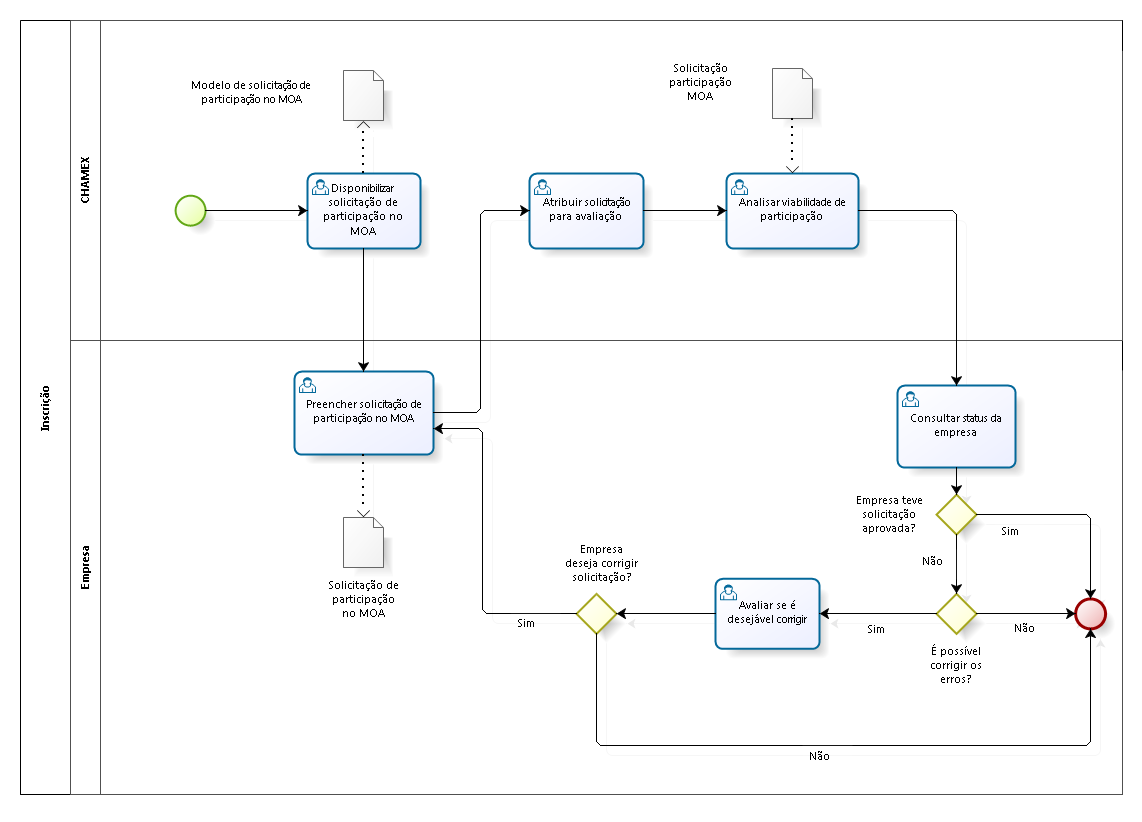
\includegraphics[scale=0.5]{to-be_5}
	\label{fig:tobeversaofinal}
	\caption[Quinta Versão (Final) do Modelo TO-BE]{Quinta Versão (Final) do Modelo TO-BE.}
\end{figure}
As três atividades incluídas são descritas da seguinte maneira:
\begin{itemize}
	\item{\textbf{Consultar \emph{Status} da Empresa}: Empresa realiza consulta no site do MOA a respeito do status da sua solicitação (aprovada ou rejeitada);}
	\item{\textbf{Avaliar se é Desejável Corrigir}: Empresa avalia com base nos resultados emitidos pelo \emph{check-list} da solicitação realizado pelo analisador do MOA se é desejável corrigir os erros com o objetivo de novamente ter sua solicitação analisado ou se é preferível não corrigir os erros e abandonar o processo de inscrição;}
	\item{\textbf{Atribuir a Solicitaçao para Avaliação}: Gerente do MOA atribui a solictação para ser validada por um analista a ser escolhido por ele.}
\end{itemize}

	\section[Definição de Metas e Indicadores para os Processos]{Definição de Metas e Indicadores para os Processos}
	\label{sec:processotobe_metas}
		TO DO

	\section[Identificação de Pontos de Automatização e Melhoria]{Identificação de Pontos de Automatização e Melhoria}
	\label{sec:processotobe_pontos}
		Levando em conta que a solicitação de participação do MOA era preenchida pela empresa antigamente via planilha Excel e conferida manualmente pelo analisador do MOA, o grupo pensou em qual processo poderia ser atacado de modo a informatizar esses passos.
\\ \indent Embora o processo tenha sofrido alterações como um todo, destacam-se o formulário \emph{web} criado para servir como solicitação de participação no MOA e o \emph{check-list} a ser utilizado pelo analisador para validar ou não a participação da empresa.
\\ \indent Os dados a serem preenchidos no formulário foram todos inseridos nesse contexto da automação, com o objetivo de também conter regras de negócio que antigamente não estavam disponíveis para verificação em tempo real na planilha Excel. Essa melhoria por si só já antecede para o preenchimento do formulário trabalhos realizados anteriormente de forma mais complexa e manual em atividades posteriores, como um campo obrigatório em branco ou violando alguma regra básica de negócio.
\\ \indent Enquanto antigamente a análise da solicitação era feita manualmente e informada à empresa pelo analisador sem o auxílio de uma ferramenta que automatizasse essa atividade, agora, com a melhoria no processo, foi criado um \emph{check-list} em que, caso haja alguma discordância com as regras de negócio identificada pelo analisador, automaticamente um e-mail é enviado à empresa que deseja participar, onde, através da consulta do status da sua solicitação, é possível ela optar em corrigir esses dados, já recuperando respostas no \emph{check-list}. Desse modo o processo de correção tornou-se menos complexo por já trazer dados anteriores preenchidos pela empresa que podem ser aproveitados, além de já apresentar ao responsável pelo preenchimento quais erros foram encontrados no \emph{check-list} realizado. 
\\ \indent A tomada de decisão quanto à corrigir ou não erros no formulário também foi identificada como um ponto de automatização, visto que rapidamente a empresa terá acesso ao formulário a ser corrigido ou abandonará o processo de inscrição.
\\ \indent Os passos descritos anteriormente passaram por um processo de automação, onde através da ferramenta Bizagi Studio o formulário, o check list e a tomada de decisão quanto à correção dos dados foi criada em uma aplicação, sendo possível visualizar através de uma solução derivada diretamente do processo modelado como este novo processo iria funcionar em um contexto real.
	%[MPR]	Realizar simulação (TO-BE) e apresentar os resultados;
		%\input{source/}
	%[RS]	Registrar os requisitos e a rastreabilidade, proposta no PGR, na ferramenta selecionada;
		%\input{source/}
	%[MPR]	Automatizar o processo redesenhado;
		%\input{source/}
	%[MPR]	Apresentar as melhorias;
		%\input{source/}
	%[MPR]	Apresentar comparação e análise entre o processo redesenhado e o processo “atual”;
		%\input{source/}
	%[MPR]	Definir Metas e indicadores para os processos;
		%\input{source/}
	%[MPR & RS]	Realizar relato de experiência (texto livre), sobre a realização do trabalho;
		%\input{source/}
	%[MPR & RS]	Lições aprendidas
		%\input{source/}
	%[MPR & RS]	Avaliação
		%\input{source/}
	%[MPR & RS]	Planejamento (Cronograma)
		%\input{source/}
	%[MPR]	Apresentar a solução de software, referente à automação do processo, sob a perspectiva de modelagem de processos
		%\input{source/}
	%[RS]	Apresentar a solução de software, referente à automação do processo, sob a perspectiva da engenharia de requisitos
		%\input{source/}

		\bibliography{bibliografia}
		
	\backmatter
		\bookmarksetup{startatroot} 
		\postextual
    		\printindex

\end{document}
